\documentclass{beamer}% usefull options [handout]
\usepackage{graphicx}
\usepackage{amsmath}
%\useoutertheme{infolines}
\usetheme{Hannover}% other nice themes Hannover, CambridgeUS, AnnArbor, Madrid, PaloAlto, Malmoe, Rochester 
\usecolortheme{beetle}% other options "dove"
\usefonttheme{structuresmallcapsserif}
\setbeamertemplate{items}[triangle] % other options "circle", "ball", "square"
%\setbeamertemplate{blocks}[rounded][shadow=true]
%\setbeamertemplate{navigation symbols}{}
%\useoutertheme[height=20pt]{sidebar}
% NOTE: this theme inverts colors, if one wants to use common colors it's necessary
% to comment the code on the chunk about lattice settings  
\setbeamercolor{normal text}{fg=white,bg=black}% inverted black background white foreground
\setbeamercolor*{palette sidebar secondary}{fg=white}

%************ Title & Author ***********************
\title[FLR in 10 slides]{FLR in 10 slides or less}
\author{Ernesto Jardim}

\usepackage{Sweave}
\begin{document}
\Sconcordance{concordance:FLRin10slides.tex:FLRin10slides.Rnw:%
1 20 1 1 0 4 1 1 6 32 1 1 24 1 2 24 1 1 2 4 0 1 3 13 1 1 2 25 0 1 2 11 %
1 1 2 20 0 1 2 12 1 1 2 25 0 1 2 11 1 1 2 27 0 1 2 7 1 1 3 2 0 2 1 1 2 %
1 0 1 1 1 2 1 0 2 1 3 0 1 2 3 1 1 3 2 0 1 1 1 2 1 0 2 1 1 2 1 0 1 2 4 0 %
1 2 3 1}

%===========================================
% some code we need 
%===========================================

%*******************************************
\begin{frame}%[plain]
\titlepage
\begin{flushright}
	
\includegraphics[width=0.1\textwidth]{cc.png}
\end{flushright}
\end{frame}

%*******************************************
% \begin{frame}
% \frametitle{Outline}
% \tableofcontents
% \end{frame}

%===========================================
% INTRODUCTION
%===========================================
\section{FLR ??}
%*******************************************
\begin{frame}
   \frametitle{What is FLR ?}
\begin{itemize}
	\item FLR = Fisheries Libraries in R
	\item FLR is a set of R packages
	\item FLR is developed and maintained by a group of fisheries scientists
\end{itemize}

\end{frame}

%*******************************************
\begin{frame}
   \frametitle{Packages}
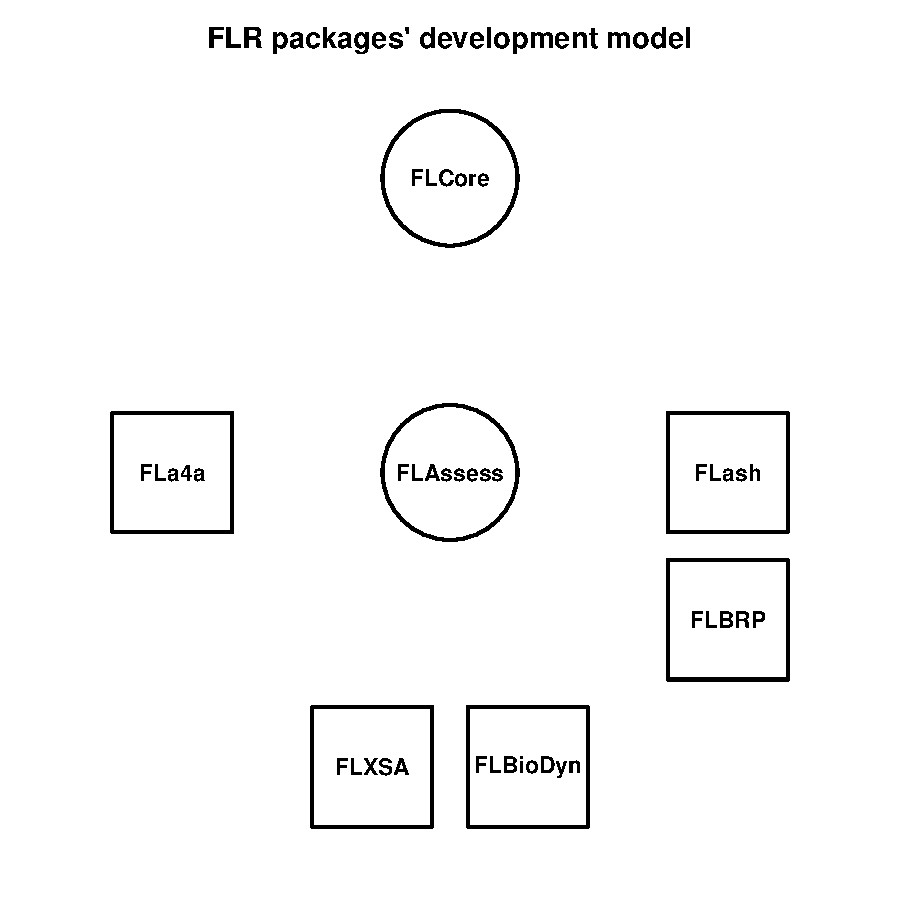
\includegraphics{FLRin10slides-002}
\end{frame}


%-------------------------------------------
% FLQuant
%-------------------------------------------
\section{FLQuant}
%*******************************************
\begin{frame}[containsverbatim]
  \frametitle{FLQuant}

Stands for "FL quantity" and it's the smallest component of FLR classes.\newline 

Six dimensional array used to store data of a particular type (e.g. catch numbers), with the follwoing dimensions:\newline

% Dimensions are:
% \begin{enumerate}
% 	\item User defined (age, length etc.)
% 	\item Year
% 	\item Unit (substocks, male/female)
% 	\item Season
% 	\item Area
% 	\item Iter
% \end{enumerate}
{\scriptsize{
\begin{Schunk}
\begin{Soutput}
[1] "quant"  "year"   "unit"   "season" "area"   "iter"  
\end{Soutput}
\end{Schunk}
}}


\end{frame}

%-------------------------------------------
% FLStock
%-------------------------------------------
\section{FLStock}
%***************************************
\begin{frame}[containsverbatim]
  \frametitle{FLStock}
Represents a fish stock and comprises a number of slots.
{\scriptsize{
\begin{Schunk}
\begin{Sinput}
> showClass("FLStock")
\end{Sinput}
\begin{Soutput}
Class "FLStock" [package "FLCore"]

Slots:
                                                                       
Name:         catch      catch.n     catch.wt     discards   discards.n
Class:      FLQuant      FLQuant      FLQuant      FLQuant      FLQuant
                                                                       
Name:   discards.wt     landings   landings.n  landings.wt        stock
Class:      FLQuant      FLQuant      FLQuant      FLQuant      FLQuant
                                                                       
Name:       stock.n     stock.wt            m          mat      harvest
Class:      FLQuant      FLQuant      FLQuant      FLQuant      FLQuant
                                                                       
Name:  harvest.spwn       m.spwn         name         desc        range
Class:      FLQuant      FLQuant    character    character      numeric

Extends: 
Class "FLS", directly
Class "FLComp", by class "FLS", distance 2
\end{Soutput}
\end{Schunk}
}}
\end{frame}

%-------------------------------------------
% FLIndex
%-------------------------------------------
\section{FLIndex}
%***************************************
\begin{frame}[containsverbatim]
  \frametitle{FLIndex}
Represents a index (e.g. index of abundance from a survey)
{\scriptsize{
\begin{Schunk}
\begin{Sinput}
> showClass("FLIndex")
\end{Sinput}
\begin{Soutput}
Class "FLIndex" [package "FLCore"]

Slots:
                                                                       
Name:          type distribution        index    index.var      catch.n
Class:    character    character      FLQuant      FLQuant      FLQuant
                                                                       
Name:      catch.wt       effort  sel.pattern      index.q         name
Class:      FLQuant      FLQuant      FLQuant      FLQuant    character
                                
Name:          desc        range
Class:    character      numeric

Extends: "FLComp"
\end{Soutput}
\end{Schunk}
}}

\end{frame}

%-------------------------------------------
% FLSR
%-------------------------------------------
\section{FLSR}
%***************************************
\begin{frame}[containsverbatim]
  \frametitle{FLSR}
Represents a stock-recruitment relationship and allows the estimation of its parameters.
{\scriptsize{
\begin{Schunk}
\begin{Sinput}
> showClass("FLSR")
\end{Sinput}
\begin{Soutput}
Class "FLSR" [package "FLCore"]

Slots:
                                                                       
Name:           rec          ssb        covar     logerror        model
Class:      FLQuant      FLQuant     FLQuants      logical      formula
                                                                       
Name:          logl           gr distribution      initial       params
Class:     function     function       factor     function        FLPar
                                                                       
Name:        logLik         vcov      hessian      details    residuals
Class:       logLik        array        array         list      FLArray
                                                          
Name:        fitted         name         desc        range
Class:      FLArray    character    character      numeric

Extends: 
Class "FLModel", directly
Class "FLComp", by class "FLModel", distance 2
\end{Soutput}
\end{Schunk}
}}
\end{frame}

%-------------------------------------------
% FLlst
%-------------------------------------------
\section{FLR Lists}
%***************************************
\begin{frame}[containsverbatim]
  \frametitle{FLlist}
A list of other classes
{\scriptsize{
\begin{Schunk}
\begin{Sinput}
> showClass("FLlst")
\end{Sinput}
\begin{Soutput}
Class "FLlst" [package "FLCore"]

Slots:
                                              
Name:      .Data     names      desc      lock
Class:      list character character   logical

Extends: 
Class "list", from data part
Class "vector", by class "list", distance 2

Known Subclasses: 
Class "FLQuants", directly
Class "FLCohorts", directly
Class "FLComps", directly
Class "FLPars", directly
Class "FLModelSims", directly
Class "FLStocks", by class "FLComps", distance 2
Class "FLIndices", by class "FLComps", distance 2
Class "FLBiols", by class "FLComps", distance 2
Class "FLSRs", by class "FLComps", distance 2
\end{Soutput}
\end{Schunk}
}}

\end{frame}

\section{Example}
%***************************************
\begin{frame}[containsverbatim]
  \frametitle{Example I}
\begin{Schunk}
\begin{Sinput}
> # load --------------------------------
> library(FLCore)
> data(ple4.index)
> data(ple4)
> # FLStock -----------------------------
> plot(ple4)
> summary(ple4)
> # FLQuant -----------------------------
> cth <- catch(ple4)
> plot(cth)
> summary(cth)
\end{Sinput}
\end{Schunk}
\end{frame}

\begin{frame}[containsverbatim]
  \frametitle{Example II}
\begin{Schunk}
\begin{Sinput}
> # FLIndex -----------------------------
> plot(ple4.index)
> summary(ple4.index)
> # FLSR --------------------------------
> ple4.sr <- as.FLSR(ple4, model="bevholt")
> ple4.sr <- fmle(ple4.sr)
> plot(ple4.sr)
> # FLlst -------------------------------
> flqs <- FLQuants(c=catch(ple4), b=stock(ple4))
> xyplot(data~year, groups=qname, data=flqs, 
+ 	 type="l")
\end{Sinput}
\end{Schunk}
\end{frame}

\end{document}

